\documentclass[11pt,a4paper]{article}
\usepackage[utf8]{inputenc}
\usepackage[T1]{fontenc}
\usepackage{lmodern}
\usepackage[french]{babel}
\usepackage[margin=2.3cm]{geometry}
\usepackage{amsmath,amssymb}
\usepackage{graphicx}
\usepackage{booktabs}
\usepackage{xcolor}
\usepackage{enumitem}
\usepackage{tikz}
\usetikzlibrary{decorations.pathmorphing,patterns}
\usepackage{tcolorbox}
\usepackage{hyperref}
\hypersetup{colorlinks=true,linkcolor=blue!50!black,urlcolor=blue!50!black}

\newcommand{\dd}{\mathrm{d}}
\newcommand{\kd}{k_1^{d}}
\newcommand{\uc}{u_c}
\newtcolorbox{alamain}{colback=yellow!8,colframe=orange!70!black,title=À faire à la main,fonttitle=\bfseries}
\newtcolorbox{idee}{colback=blue!5,colframe=blue!50!black,title=L'idée à retenir,fonttitle=\bfseries}

\title{Deux ressorts en série dont un endommageable :\\
comprendre le snap-back, la solution analytique,\\
le calcul statique et le calcul dynamique}
\author{Note pédagogique, dépôt \texttt{1D\_damage\_spring\_system}}
\date{\today}

\begin{document}
\maketitle

\tableofcontents
\clearpage

\section{Le système et les ordres de grandeur}

\subsection{Le montage}
On modélise un essai de traction sur une éprouvette de béton montée dans une machine dont la
chaîne de chargement n'est pas infiniment rigide. Le modèle le plus simple possible est une
chaîne de deux ressorts :

\begin{center}
\begin{tikzpicture}[scale=1.1]
  \fill[pattern=north east lines] (-0.4,-0.5) rectangle (0,0.5);
  \draw[thick] (0,-0.5) -- (0,0.5);
  \draw[thick,decorate,decoration={zigzag,segment length=6pt,amplitude=3pt}] (0,0) -- (3,0);
  \node[above] at (1.5,0.25) {ressort 1 : béton, $\kd(u_1)$};
  \draw[thick,fill=gray!30] (3,-0.35) rectangle (3.8,0.35);
  \node at (3.4,0) {$m_1$};
  \draw[thick,decorate,decoration={zigzag,segment length=6pt,amplitude=3pt}] (3.8,0) -- (6.8,0);
  \node[above] at (5.3,0.25) {ressort 2 : acier, $k_2$};
  \draw[thick] (6.8,-0.4) -- (6.8,0.4);
  \draw[->,thick,red] (6.8,0) -- (7.8,0) node[right] {$u_2(t)$ imposé};
  \node[below] at (0,-0.6) {noeud 0};
  \node[below] at (3.4,-0.5) {noeud 1 : $u_1$ inconnu};
  \node[below] at (6.8,-0.5) {noeud 2};
\end{tikzpicture}
\end{center}

\begin{itemize}[nosep]
  \item Le \textbf{ressort 1} représente l'éprouvette de béton : longueur $L_1 = 100$~mm, section
        $A_1 = 100\times100$~mm$^2$, module $E_1 = 30\,000$~MPa. Il s'endommage en traction.
  \item Le \textbf{ressort 2} représente la barre d'acier de la chaîne de chargement : longueur
        $L_2 = 1000$~mm, diamètre 20~mm ($A_2 = 314$~mm$^2$), module $E_2 = 210\,000$~MPa. Il
        reste élastique.
  \item Le \textbf{noeud 1} porte la masse concentrée $m_1$ (demi-éprouvette, demi-barre, mors) ;
        c'est le seul degré de liberté inconnu.
  \item Le \textbf{noeud 2} est piloté en déplacement : on impose $u_2(t)$ croissant.
\end{itemize}
Unités : N, mm, s. Alors les contraintes sont en MPa et les masses en tonnes.

\subsection{Les raideurs}
Une barre élastique de longueur $L$, section $A$, module $E$ soumise à une force $F$ s'allonge de
$\delta = FL/(EA)$ : c'est un ressort de raideur
\begin{equation}
  k = \frac{EA}{L}.
\end{equation}
\begin{alamain}
$k_1 = \dfrac{30\,000\times10\,000}{100} = 3{,}0\cdot10^6$~N/mm, \quad
$k_2 = \dfrac{210\,000\times314{,}16}{1000} = 6{,}6\cdot10^4$~N/mm, \quad
$\dfrac{k_2}{k_1} = 0{,}022$.
\end{alamain}
La barre d'acier est donc \emph{45 fois plus souple} que l'éprouvette intacte, parce qu'elle est
dix fois plus longue et trente fois moins large. Retenons ce rapport : tout le snap-back vient de là.

\section{La loi d'endommagement du ressort 1}

\subsection{Raideur sécante et variable d'endommagement}
On note $d\in[0,1]$ l'endommagement : $d = 0$ matériau sain, $d = 1$ matériau rompu. La raideur
effective du ressort 1 est la raideur \emph{sécante}
\begin{equation}
  \kd = k_1(1-d),\qquad F_1 = \kd\,u_1 = k_1(1-d)\,u_1 .
\end{equation}
On choisit la loi
\begin{equation}
  d(\kappa) = 1-\exp\!\left(-\frac{\kappa^2}{\uc^2}\right),\qquad
  \kappa(t) = \max_{\tau\le t}u_1(\tau).
  \label{eq:loi}
\end{equation}
La variable d'histoire $\kappa$ garantit l'\textbf{irréversibilité} : si $u_1$ diminue (décharge),
$\kappa$ ne bouge pas, $d$ reste figé et le ressort décharge élastiquement avec la raideur
$k_1(1-d)$. Tant que le chargement est monotone, $\kappa = u_1$ et on peut écrire $d(u_1)$.

\subsection{La courbe force--allongement du ressort 1}
En charge, avec $x = u_1/\uc$ :
\begin{equation}
  F_1(u_1) = k_1\,u_1\,e^{-x^2}.
  \label{eq:F1}
\end{equation}
Cette courbe monte, passe par un maximum, puis redescend vers zéro : c'est un comportement
\emph{adoucissant}. Trois points caractéristiques se calculent à la main.

\paragraph{Le pic.} On dérive \eqref{eq:F1} (produit $u_1\times e^{-x^2}$, avec $\dd x/\dd u_1 = 1/\uc$) :
\begin{equation}
  \frac{\dd F_1}{\dd u_1} = k_1e^{-x^2} + k_1u_1\Bigl(-\frac{2u_1}{\uc^2}\Bigr)e^{-x^2}
  = k_1e^{-x^2}\bigl(1-2x^2\bigr).
  \label{eq:dF1}
\end{equation}
Elle s'annule pour $x = 1/\sqrt2$, soit
\begin{equation}
  u_1^{\text{pic}} = \frac{\uc}{\sqrt2},\qquad
  F_{\max} = k_1\frac{\uc}{\sqrt2}e^{-1/2} = \frac{k_1\uc}{\sqrt{2e}},\qquad
  d^{\text{pic}} = 1-e^{-1/2} = 0{,}393 .
\end{equation}
Au pic, le ressort a déjà perdu 39~\% de sa raideur : le pic de force n'est pas le début de
l'endommagement, c'est le moment où la perte de raideur l'emporte sur l'augmentation
d'allongement.

\paragraph{La pente descendante la plus raide.} Elle joue un rôle central pour le snap-back. On
dérive une seconde fois :
\begin{equation}
  \frac{\dd^2F_1}{\dd u_1^2} = \frac{k_1}{\uc}e^{-x^2}\bigl[-2x(1-2x^2) - 4x\bigr]
  = \frac{k_1}{\uc}e^{-x^2}\,2x\bigl(2x^2-3\bigr),
\end{equation}
nulle pour $x^2 = 3/2$. En ce point d'inflexion la pente vaut
\begin{equation}
  \left.\frac{\dd F_1}{\dd u_1}\right|_{x=\sqrt{3/2}} = k_1e^{-3/2}(1-3) = -2e^{-3/2}k_1 = -0{,}446\,k_1 .
  \label{eq:pentemax}
\end{equation}
\begin{idee}
Le ressort endommageable ne peut jamais « décharger » plus vite que $-0{,}446\,k_1$ par unité
d'allongement. C'est ce nombre qu'il faut comparer à $k_2$.
\end{idee}

\paragraph{L'énergie dissipée totale.} Le travail pour rompre complètement le ressort est l'aire
sous la courbe :
\begin{equation}
  \int_0^\infty k_1u\,e^{-u^2/\uc^2}\,\dd u = k_1\Bigl[-\frac{\uc^2}{2}e^{-u^2/\uc^2}\Bigr]_0^\infty
  = \frac{k_1\uc^2}{2}.
\end{equation}
Rapportée à la section, c'est l'énergie de rupture $G_f = k_1\uc^2/(2A_1)$ (en N/mm, c'est-à-dire
des J/m$^2$ à un facteur 1000 près).

\subsection{Calibration de $\uc$ sur la résistance en traction}
On veut que le pic de force corresponde à la résistance en traction du béton, $F_{\max} = f_tA_1$
avec $f_t = 3$~MPa :
\begin{equation}
  \uc = \frac{\sqrt{2e}\,f_tA_1}{k_1} = \frac{\sqrt{2e}\,f_tL_1}{E_1}.
\end{equation}
\begin{alamain}
$\uc = \dfrac{2{,}3316\times3\times100}{30\,000} = 0{,}0233$~mm, \quad
$u_1^{\text{pic}} = 0{,}0165$~mm (soit une déformation $1{,}65\cdot10^{-4}$, réaliste pour un béton),\\
$F_{\max} = 30\,000$~N, \quad
$G_f = \dfrac{3\cdot10^6\times0{,}0233^2}{2\times10^4} = 0{,}082$~N/mm.
\end{alamain}
Remarque utile : en combinant, $G_f = e\,f_t^2L_1/E_1$. À $f_t$ et $G_f$ donnés, la longueur $L_1$
sur laquelle on « étale » l'endommagement n'est pas libre. Ici 100~mm donne 0{,}082~N/mm, dans
la plage du béton courant (0{,}08 à 0{,}1~N/mm) : le modèle à un seul ressort est cohérent
énergétiquement. Si l'on découpait l'éprouvette en plusieurs ressorts, un seul s'endommagerait
et il faudrait réduire $\uc$ avec sa longueur pour conserver $G_f$ (c'est la « bande de
fissuration » de Bažant et de Borst).

\section{L'équilibre statique et la construction graphique}

\subsection{L'équation d'équilibre}
Le noeud 1 est tiré vers la gauche par le ressort 1 avec la force $F_1 = \kd u_1$ et vers la
droite par le ressort 2 avec la force $F_2 = k_2(u_2-u_1)$. À l'équilibre (sans masse, ou à
vitesse nulle) :
\begin{equation}
  \boxed{\;\kd(u_1)\,u_1 = k_2\,(u_2-u_1)\;}
  \qquad\Longleftrightarrow\qquad
  R(u_1;u_2) \equiv \bigl(\kd(u_1)+k_2\bigr)u_1 - k_2u_2 = 0 .
  \label{eq:eq}
\end{equation}
La force mesurée par la machine est $F = F_2 = k_2(u_2-u_1)$, égale à $F_1$ à l'équilibre.

\subsection{Lecture graphique}
Dans le plan $(u_1, F)$ :
\begin{itemize}[nosep]
  \item le membre de gauche de \eqref{eq:eq} est la \textbf{courbe} $F_1(u_1)$ du ressort 1 ;
  \item le membre de droite est une \textbf{droite} de pente $-k_2$ qui coupe l'axe des abscisses en
        $u_1 = u_2$ et l'axe des ordonnées en $k_2u_2$.
\end{itemize}
Les équilibres sont les intersections. Quand on augmente $u_2$, la droite se translate vers la
droite sans changer de pente (figure~\ref{fig:constr}, gauche).

\begin{figure}[h]\centering
  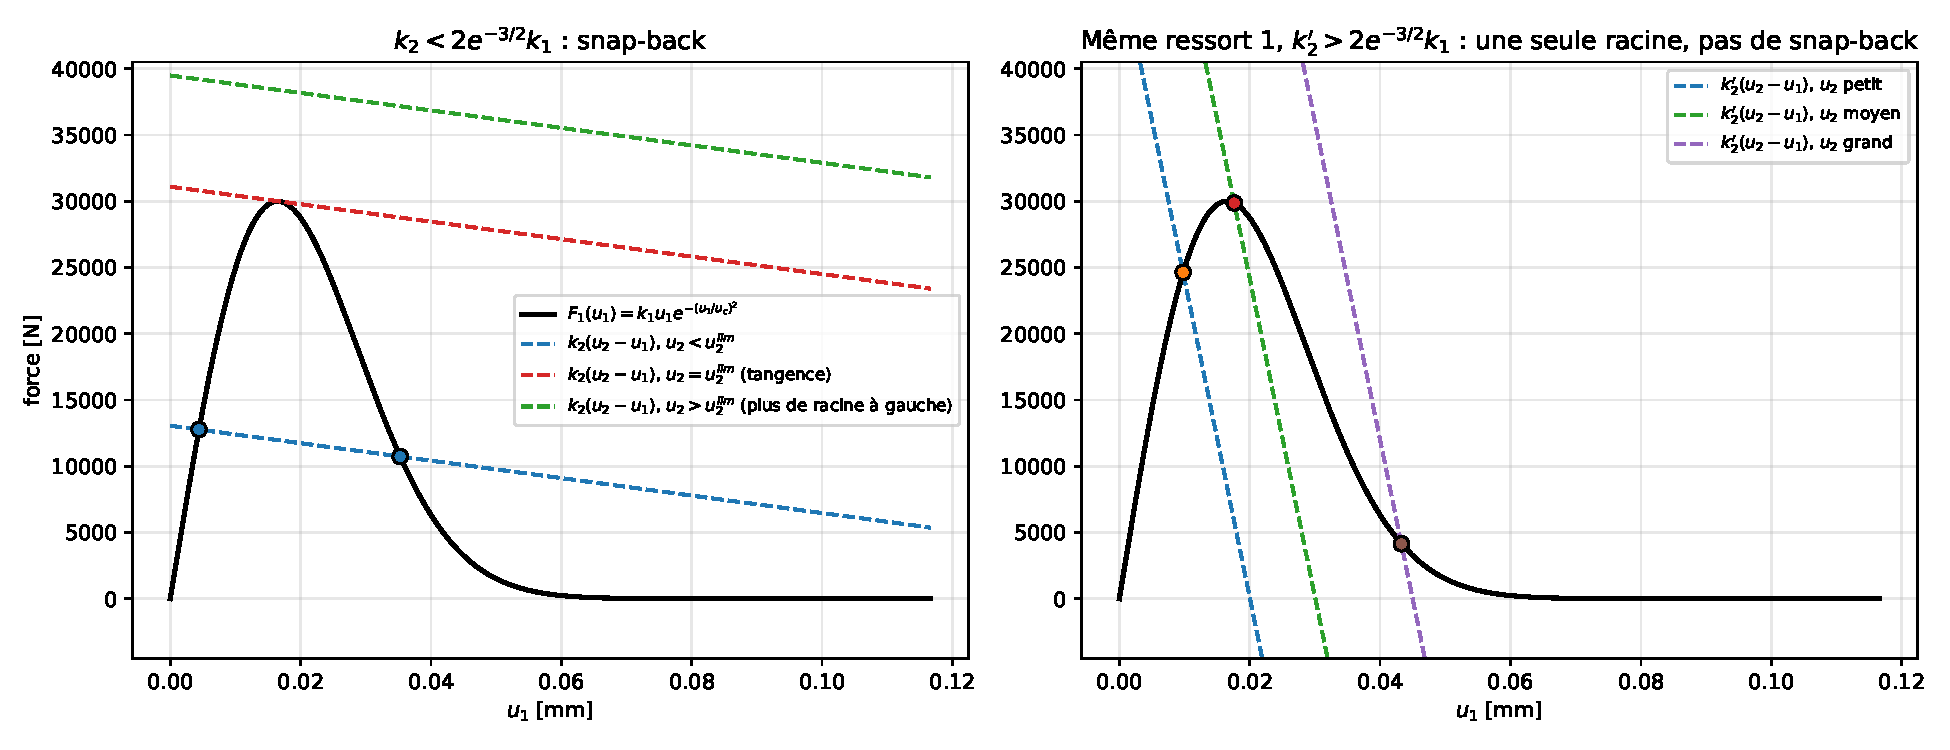
\includegraphics[width=\textwidth]{figures/explication_construction.pdf}
  \caption{Construction graphique de l'équilibre. Gauche : avec la barre d'acier de 1~m, la
  droite est presque plate ($k_2 \ll k_1$) ; dès que $u_2$ dépasse $0{,}471$~mm elle passe
  au-dessus du pic et il n'y a plus d'intersection sur la branche montante : saut. Droite : avec
  un ressort 2 raide ($k_2' = 0{,}8\,k_1$), la droite est plus pentue que la descente la plus raide de
  $F_1$ ; une seule intersection quel que soit $u_2$, pas de saut.}
  \label{fig:constr}
\end{figure}

Trois situations, selon $u_2$, dans le cas de gauche :
\begin{enumerate}[nosep]
  \item $u_2$ petit (droite bleue) : une intersection sur la branche montante de $F_1$ (stable)
        et une sur la branche descendante loin à droite (que l'on n'atteint pas en chargeant depuis
        zéro). Le système suit la première.
  \item $u_2 = u_2^{\lim}$ (droite rouge) : la droite est \emph{tangente} à $F_1$ juste après le pic.
        C'est le \textbf{point limite}.
  \item $u_2 > u_2^{\lim}$ (droite verte) : plus aucune intersection à gauche. Le seul équilibre
        est très loin à droite, sur la branche $F_1\simeq0$, c'est-à-dire $u_1 \simeq u_2$ : le
        ressort 1 est rompu et le ressort 2 détendu. Le système doit \textbf{sauter} jusque-là.
\end{enumerate}

\subsection{Pourquoi la tangence ?}
Sur la branche descendante de $F_1$, l'intersection avec la droite persiste tant que la courbe
descend \emph{moins vite} que la droite, c'est-à-dire tant que $\dd F_1/\dd u_1 > -k_2$. Le point
limite est atteint quand
\begin{equation}
  \frac{\dd F_1}{\dd u_1} = -k_2
  \quad\Longleftrightarrow\quad
  k_t(u_1) \equiv \frac{\dd F_1}{\dd u_1} + k_2 = k_1e^{-x^2}(1-2x^2) + k_2 = 0 .
  \label{eq:kt}
\end{equation}
La quantité $k_t$ est la \textbf{raideur tangente du système} : c'est la dérivée du résidu
$R$ par rapport à $u_1$, et c'est elle qui apparaîtra dans le Newton--Raphson.

\section{Snap-back ou pas : le critère}

\subsection{Le critère en raideurs}
L'équation \eqref{eq:kt} n'a de solution que si la droite peut être tangente à la descente de
$F_1$, donc si sa pente $-k_2$ est moins raide que la pente minimale \eqref{eq:pentemax} :
\begin{equation}
  \boxed{\;\text{snap-back}\iff k_2 < 2e^{-3/2}\,k_1 \simeq 0{,}446\,k_1\;}
  \label{eq:crit}
\end{equation}
Si au contraire $k_2 > 0{,}446\,k_1$, la droite coupe toujours $F_1$ en un seul point : la réponse
$F(u_2)$ est adoucissante mais \emph{régulière}, et un pilotage en déplacement la suit sans
difficulté (figure~\ref{fig:constr}, droite).

\subsection{Le critère en longueurs et sections}
En remplaçant les raideurs par $EA/L$ :
\begin{equation}
  \frac{E_2A_2}{L_2} < 0{,}446\,\frac{E_1A_1}{L_1}
  \quad\Longleftrightarrow\quad
  L_2 > \frac{1}{0{,}446}\,\frac{E_2A_2}{E_1A_1}\,L_1 = 2{,}24\,\frac{E_2A_2}{E_1A_1}\,L_1 .
\end{equation}
\begin{alamain}
$E_1A_1 = 3{,}0\cdot10^8$~N, $E_2A_2 = 6{,}6\cdot10^7$~N, rapport $0{,}22$.\\
$L_2^{\text{crit}} = 2{,}24\times0{,}22\times100 = 49$~mm.
\end{alamain}
Avec une barre d'acier de 1~m on est vingt fois au-delà : snap-back certain. Pour l'éviter il
faudrait une chaîne de chargement de moins de 5~cm de long (irréaliste), ou une section d'acier
vingt fois plus grande (diamètre 90~mm), ou une éprouvette vingt fois plus longue (2~m, mais alors
l'endommagement se localiserait dans une partie de l'éprouvette et le reste, élastique, jouerait le
rôle du ressort 2 : le problème se reproduit à l'intérieur de l'éprouvette).

\subsection{Interprétation énergétique}
Au-delà du pic, le ressort 1 rend de l'énergie quand on le laisse s'allonger (sa force décroît),
et le ressort 2 rend aussi de l'énergie quand il se détend. Si le ressort 2 est très souple, il a
stocké beaucoup d'énergie, $\tfrac12F_{\max}^2/k_2$, que le ressort 1 adoucissant est incapable
d'absorber. Le surplus ne peut partir qu'en énergie cinétique : c'est le saut.
\begin{alamain}
Énergie dans la barre d'acier au pic : $\dfrac{30\,000^2}{2\times65\,973} = 6\,820$~N.mm = 6{,}8~J.\\
Énergie dans le béton au pic : $\tfrac12F_{\max}u_1^{\text{pic}} = \tfrac12\times30\,000\times0{,}0165 = 247$~N.mm = 0{,}25~J.
\end{alamain}
La barre contient 27 fois plus d'énergie que l'éprouvette. Voilà le snap-back expliqué sans
équation.

\subsection{Les trois régimes}
\begin{center}
\begin{tabular}{@{}lll@{}}
\toprule
Pilotage & Jusqu'où peut-on aller ? & Ce qui bloque\\
\midrule
en force & jusqu'au pic $F_{\max}$ & au-delà, aucun équilibre statique quel que soit $k_2$\\
en déplacement, $k_2 > 0{,}446k_1$ & toute la courbe & rien : branche adoucissante régulière\\
en déplacement, $k_2 < 0{,}446k_1$ & jusqu'au point limite $u_2^{\lim}$ & la branche rebrousse chemin en $u_2$\\
\bottomrule
\end{tabular}
\end{center}
Le point limite en déplacement ($k_t = 0$) est très proche du pic en force ($\dd F_1/\dd u_1 = 0$)
quand $k_2 \ll k_1$ : ici $x_{\lim} = 0{,}720$ contre $x_{\text{pic}} = 0{,}707$.

\section{La solution analytique}

\subsection{Paramétrer par $u_1$ au lieu de $u_2$}
Résoudre \eqref{eq:eq} en $u_1$ à $u_2$ donné est impossible en forme fermée (équation
transcendante). Mais \eqref{eq:eq} est \emph{linéaire en $u_2$} : on l'inverse donc dans l'autre
sens.
\begin{equation}
  \boxed{\;u_2(u_1) = u_1\Bigl(1+\frac{k_1}{k_2}e^{-x^2}\Bigr),\qquad
  F(u_1) = k_1u_1e^{-x^2}\;}
  \label{eq:ana}
\end{equation}
En faisant croître $u_1$ de 0 à l'infini on décrit toute la courbe $F(u_2)$, y compris la
partie que l'expérience ne peut pas suivre.

\subsection{Où $u_2$ rebrousse chemin}
\begin{equation}
  \frac{\dd u_2}{\dd u_1} = 1 + \frac{k_1}{k_2}e^{-x^2}(1-2x^2) = \frac{k_t(u_1)}{k_2}.
\end{equation}
On retrouve la tangente du système : $u_2$ croît tant que $k_t > 0$, décroît quand $k_t < 0$.
Le point limite est la première racine de $k_t = 0$, soit
\begin{equation}
  e^{-x^2}\bigl(2x^2-1\bigr) = \frac{k_2}{k_1} = 0{,}022 .
\end{equation}
\begin{alamain}
Résolution par essais : $x = 0{,}71 \to 0{,}0050$ ; $x = 0{,}72 \to 0{,}0221$ ; $x = 0{,}73 \to 0{,}0393$.
Donc $x_{\lim} \simeq 0{,}720$, $u_1^{\lim} = 0{,}0168$~mm, et
$u_2^{\lim} = 0{,}0168\bigl(1 + 45{,}5\,e^{-0{,}518}\bigr) = 0{,}471$~mm.\\
Seconde racine (fin de la zone $k_t<0$) : $x = 2{,}50$, $u_1 = 0{,}0583$~mm, $u_2 = 0{,}0634$~mm.
\end{alamain}
La branche d'équilibre part donc de l'origine, monte jusqu'à $(u_2, F) = (0{,}471, 30\,000)$,
\emph{revient en arrière} jusqu'à $u_2 = 0{,}063$~mm en descendant à $F = 333$~N, puis repart vers la
droite le long de $F \simeq 0$, $u_2 \simeq u_1$. C'est la courbe rouge de la
figure~\ref{fig:fu}.

\begin{figure}[h]\centering
  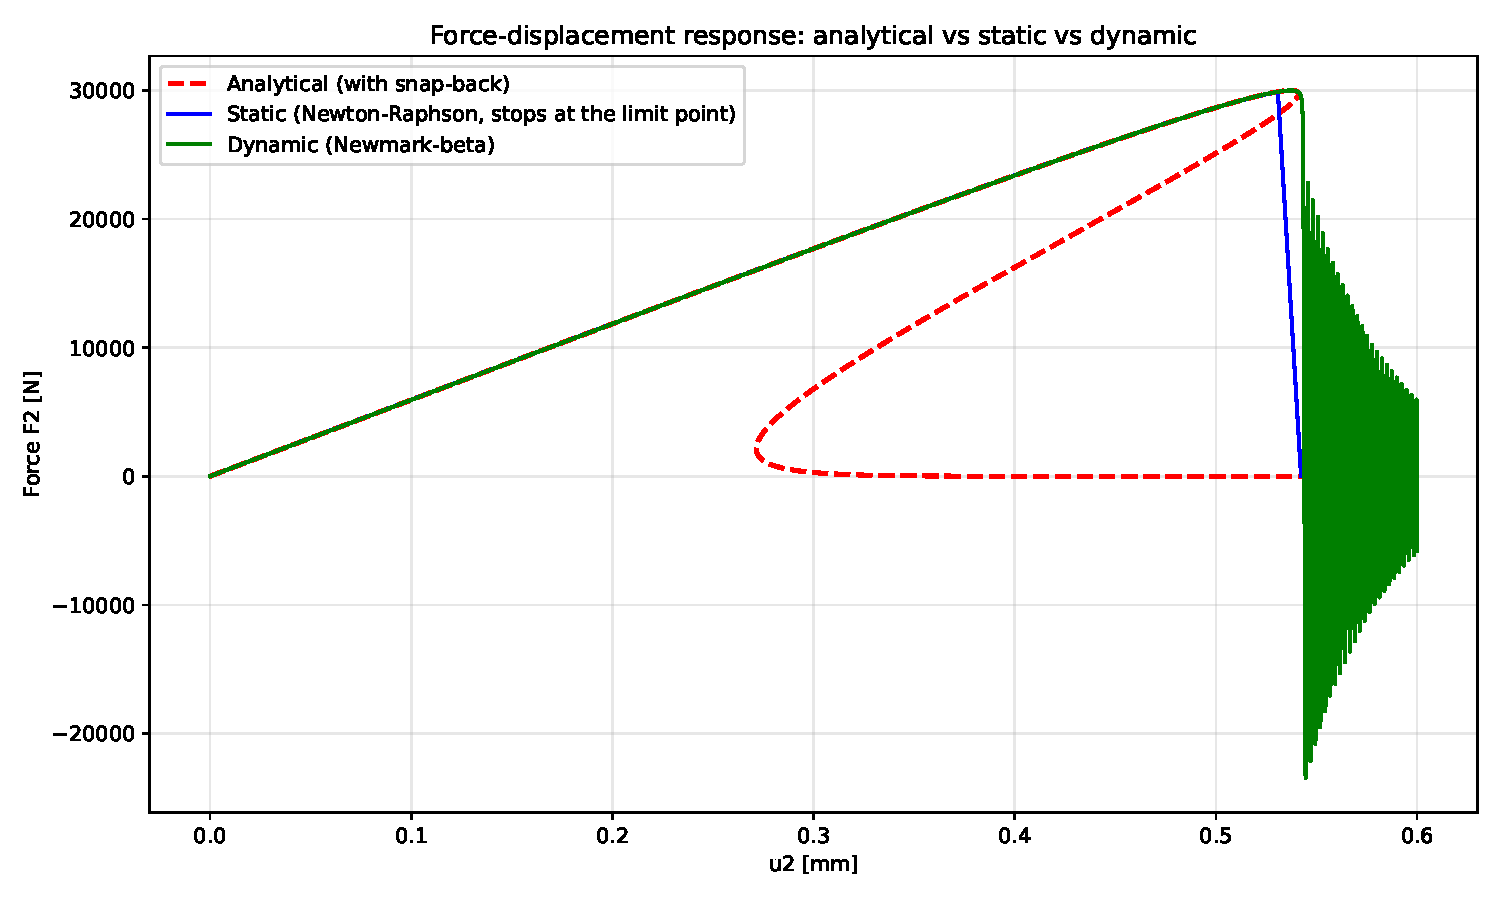
\includegraphics[width=.8\textwidth]{figures/force_displacement.pdf}
  \caption{Les trois solutions dans le plan $(u_2, F)$. Rouge : branche analytique complète avec
  son rebroussement. Bleu : statique, saut vertical au point limite. Vert : dynamique, le noeud
  oscille après la rupture et $F$ devient alternativement négative.}
  \label{fig:fu}
\end{figure}

\subsection{Le bilan d'énergie du saut}
Énergie libre du système (élastique stockée) :
\begin{equation}
  \Psi = \tfrac12k_1(1-d)u_1^2 + \tfrac12k_2(u_2-u_1)^2 .
\end{equation}
Différentions, en utilisant l'équilibre $k_1(1-d)u_1 = k_2(u_2-u_1) = F$ :
\begin{align}
  \dd\Psi &= k_1(1-d)u_1\,\dd u_1 - \tfrac12k_1u_1^2\,\dd d + k_2(u_2-u_1)(\dd u_2-\dd u_1)\\
          &= F\,\dd u_1 - Y\,\dd d + F\,\dd u_2 - F\,\dd u_1 = F\,\dd u_2 - Y\,\dd d,
\end{align}
avec $Y = \tfrac12k_1u_1^2$ le taux de restitution d'énergie. Donc, le long de la branche
d'équilibre entre deux états,
\begin{equation}
  \underbrace{\int F\,\dd u_2}_{W\ \text{(travail de la machine)}} = \Psi_2-\Psi_1 + \underbrace{\int Y\,\dd d}_{\mathcal D\ \text{(dissipé par endommagement)}} .
\end{equation}
Lors du saut réel, $u_2$ ne bouge pas, donc la machine ne fournit aucun travail. Entre l'état
« point limite » (1) et l'état « rompu au même $u_2$ » (2), on a $\Psi_1 > \Psi_2$ et l'énergie
libérée se décompose en
\begin{equation}
  \Psi_1-\Psi_2 = \mathcal D_{\text{branche}} + |W| ,
\end{equation}
où $|W|$ est l'aire comprise entre le segment vertical du saut et la branche analytique. Cette
aire est ce que le béton n'arrive pas à dissiper : elle part en énergie cinétique.
\begin{alamain}
$\Psi_1 = 247 + 6\,820 = 7\,067$~N.mm, $\Psi_2 \simeq 0$. Numériquement $\mathcal D_{\text{branche}} = 744$~N.mm
et $|W| = 6\,321$~N.mm $= 6{,}3$~J.\\
Vitesse que prendrait la masse si tout partait en cinétique : $v = \sqrt{2\times6\,321/0{,}0274} = 680$~mm/s.
\end{alamain}

\section{Le calcul statique par Newton--Raphson}

\subsection{L'algorithme}
On impose $u_2$ par petits incréments ($2000$ pas de $0$ à $0{,}6$~mm). À chaque incrément on cherche
$u_1$ tel que $R(u_1;u_2) = 0$ par la méthode de Newton :
\begin{equation}
  u_1^{(i+1)} = u_1^{(i)} - \frac{R(u_1^{(i)})}{k_t(u_1^{(i)})},\qquad
  k_t = \frac{\partial R}{\partial u_1} = \kd + u_1\frac{\dd\kd}{\dd u_1} + k_2 ,
\end{equation}
en partant de la solution de l'incrément précédent (\emph{warm start}). On arrête quand
$|R| \le 10^{-6}$~N. Géométriquement : on trace la tangente au résidu au point courant et on
prend son intersection avec l'axe.

\subsection{Ce qui se passe loin du point limite}
Le résidu est presque une droite de pente $k_t \simeq k_1+k_2$, Newton converge en deux ou trois
itérations, quadratiquement (le résidu est divisé par un facteur $\sim10^3$ à chaque itération) :
\begin{center}
\begin{tabular}{@{}lrr@{}}
\toprule
incrément 1000, $u_2 = 0{,}30015$~mm & $u_1^{(i)}$ [mm] & $R$ [N]\\
\midrule
$i=0$ (solution précédente) & 0,007056 & $-19{,}8$\\
$i=1$ & 0,007065 & $-7{,}4\cdot10^{-3}$\\
$i=2$ & 0,007065 & $-1{,}0\cdot10^{-9}$\\
\bottomrule
\end{tabular}
\end{center}

\subsection{Ce qui se passe au point limite}
Juste avant : $u_2 = 0{,}47124$~mm, il reste une racine mais $k_t$ est presque nul, Newton a besoin
de 4 itérations. Juste après : $u_2 = 0{,}47154$~mm, \emph{il n'y a plus de racine} près du point de
départ. Le résidu a l'allure de la figure~\ref{fig:resnr} : un maximum local légèrement
\emph{négatif} à $u_1 \simeq 0{,}0167$~mm, puis une descente, puis une remontée lente jusqu'à la vraie
racine en $u_1 = u_2 = 0{,}4715$~mm. Newton, parti juste à gauche du maximum, rebondit indéfiniment
autour de lui :
\begin{center}
\begin{tabular}{@{}lrrrrrrr@{}}
\toprule
$i$ & 0 & 1 & 2 & 3 & 4 & 5 & 6\\
$u_1^{(i)}$ [mm] & 0,016508 & 0,016830 & 0,015562 & 0,016518 & 0,016843 & 0,015855 & 0,016518\\
$R$ [N] & $-19{,}8$ & $-11{,}4$ & $-1\,802$ & $-19{,}2$ & $-11{,}5$ & $-1\,249$ & $-19{,}2$\\
\bottomrule
\end{tabular}
\end{center}
On reconnaît le cycle de période 3 : près du sommet la tangente est presque horizontale et
envoie l'itéré loin à gauche, d'où il revient. Au bout de 50 itérations on déclare l'échec.

\begin{figure}[h]\centering
  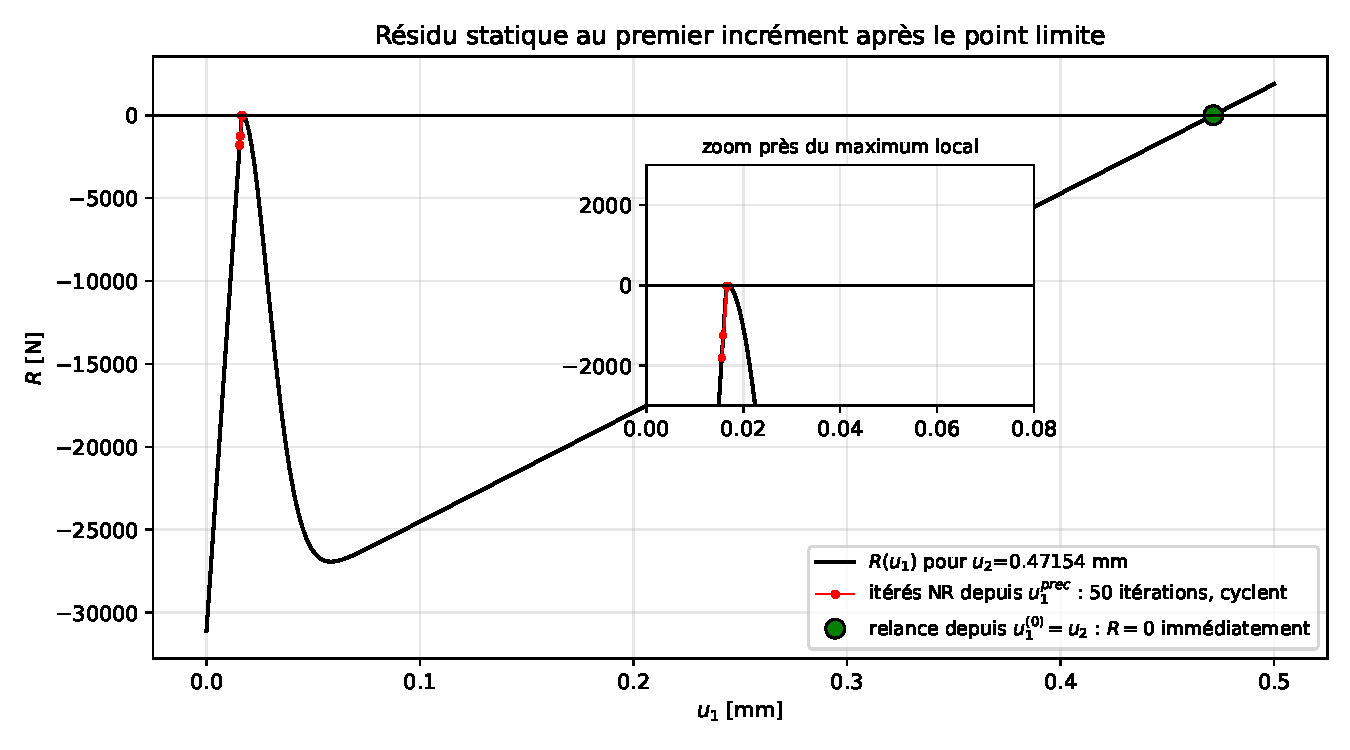
\includegraphics[width=.85\textwidth]{figures/explication_residu_nr.pdf}
  \caption{Résidu statique au premier incrément après le point limite. Les itérés de Newton
  partis de la solution précédente (rouge) cyclent autour du maximum local, sous l'axe. La
  relance depuis $u_1 = u_2$ (vert) tombe directement sur la racine : $R(u_2) = k_1u_2e^{-(u_2/\uc)^2}$
  avec $(u_2/\uc)^2 = 408$, soit un zéro à la précision machine.}
  \label{fig:resnr}
\end{figure}

\subsection{Le remède : relancer depuis l'autre branche}
Puisque la seule racine est sur la branche rompue, on relance Newton depuis $u_1^{(0)} = u_2$.
Là, le résidu est strictement croissant (pente $k_2$) et Newton converge immédiatement. Le
calcul statique reproduit ainsi le saut : la courbe bleue de la figure~\ref{fig:fu} descend
verticalement de $F_{\max}$ à $0$ au premier incrément après $u_2^{\lim}$. C'est exactement la
méthode de Sepasdar et Shakiba (2020) pour les zones cohésives ; l'alternative classique est la
méthode de longueur d'arc, qui suit la branche en faisant décroître $u_2$, ce que l'on a déjà
sous forme analytique avec \eqref{eq:ana}.

\begin{idee}
L'échec du Newton--Raphson au point limite n'est pas un défaut de précision ni de pas : c'est un
défaut de \emph{point de départ}. Raffiner les incréments rapproche seulement le point de départ
du sommet du résidu, cela ne crée pas de racine.
\end{idee}

\section{Le calcul dynamique}

\subsection{Pourquoi la dynamique ?}
Physiquement, le saut est un événement dynamique : au point limite, si l'on continue d'augmenter
$u_2$, le bilan de puissance
\begin{equation}
  \dot\Psi + \dot K = F\dot u_2 - Y\dot d
\end{equation}
ne peut être satisfait qu'avec $\dot K > 0$ : la masse accélère. Il faut donc ajouter l'inertie au
noeud 1 :
\begin{equation}
  \boxed{\;m_1\ddot u_1 + \kd(u_1)\,u_1 - k_2\bigl(u_2(t)-u_1\bigr) = 0\;}
  \label{eq:mvt}
\end{equation}
où $u_2(t) = v_2t$ est une rampe lente ($v_2 = 1$~mm/s), puis un maintien.

\subsection{Le schéma de Newmark, construit à la main}
On cherche $u_{n+1}$, $v_{n+1}$, $a_{n+1}$ à l'instant $t_{n+1} = t_n+\Delta t$. Des développements de
Taylor avec une accélération interpolée entre $a_n$ et $a_{n+1}$ donnent
\begin{align}
  u_{n+1} &= u_n + \Delta t\,v_n + \Delta t^2\Bigl[\bigl(\tfrac12-\beta\bigr)a_n + \beta\,a_{n+1}\Bigr],\\
  v_{n+1} &= v_n + \Delta t\Bigl[(1-\gamma)a_n + \gamma\,a_{n+1}\Bigr].
\end{align}
On sépare ce qui est connu (les \emph{prédicteurs}) de ce qui dépend de l'inconnue $a_{n+1}$ :
\begin{equation}
  \tilde u = u_n + \Delta t\,v_n + \tfrac{\Delta t^2}{2}(1-2\beta)a_n,\qquad
  \tilde v = v_n + (1-\gamma)\Delta t\,a_n,
\end{equation}
\begin{equation}
  u_{n+1} = \tilde u + \beta\Delta t^2a_{n+1}
  \ \Longrightarrow\
  a_{n+1} = c_1\,(u_{n+1}-\tilde u),\quad c_1 = \frac{1}{\beta\Delta t^2},\qquad
  v_{n+1} = \tilde v + \gamma\Delta t\,a_{n+1}.
\end{equation}
Avec $\beta = 1/4$, $\gamma = 1/2$ (accélération moyenne) le schéma est inconditionnellement stable et
ne dissipe pas ; avec $\gamma > 1/2$ il amortit numériquement les hautes fréquences (il faut alors
$\beta \ge (\gamma+\tfrac12)^2/4$). Le code utilise $\beta = 0{,}3$, $\gamma = 0{,}55$, légèrement
dissipatif.

\subsection{Le résidu dynamique}
On reporte $a_{n+1} = c_1(u_{n+1}-\tilde u)$ dans \eqref{eq:mvt} écrite en $t_{n+1}$ :
\begin{equation}
  \boxed{\;r(u_1) = m_1c_1\,(u_1-\tilde u) + \underbrace{\bigl(\kd(u_1)+k_2\bigr)u_1 - k_2u_2^{n+1}}_{R(u_1;u_2^{n+1})\ \text{(résidu statique)}}\;}
  \qquad
  \frac{\partial r}{\partial u_1} = m_1c_1 + k_t(u_1).
  \label{eq:rdyn}
\end{equation}
Le résidu dynamique est le résidu statique auquel on ajoute une \textbf{droite} de pente $m_1c_1$
passant par $\tilde u$. Tout est là.

\subsection{Pourquoi le Newton--Raphson passe le snap-back}
La tangente dynamique vaut $m_1c_1 + k_t$. Le résidu dynamique est strictement croissant, donc
n'a qu'une racine, dès que
\begin{equation}
  m_1c_1 > -\min k_t = 2e^{-3/2}k_1 - k_2
  \quad\Longleftrightarrow\quad
  \Delta t < \Delta t_{\max} = \sqrt{\frac{m_1}{\beta\,(2e^{-3/2}k_1-k_2)}} .
  \label{eq:dtmax}
\end{equation}
\begin{alamain}
$2e^{-3/2}k_1 - k_2 = 1{,}339\cdot10^6 - 0{,}066\cdot10^6 = 1{,}273\cdot10^6$~N/mm.\\
$m_1 = 0{,}5\times2{,}4\cdot10^{-9}\times10^4\times100 + 0{,}5\times7{,}85\cdot10^{-9}\times314\times1000 + 0{,}025 = 0{,}0274$~t.\\
$\Delta t_{\max} = \sqrt{0{,}0274/(0{,}3\times1{,}273\cdot10^6)} = 2{,}7\cdot10^{-4}$~s $= 0{,}27$~ms.\\
Période propre du système sain : $T_0 = 2\pi\sqrt{m_1/(k_1+k_2)} = 0{,}594$~ms, donc il suffit de
$N = T_0/\Delta t > 2{,}2$ pas par période. Le code prend $N = 5$, $\Delta t = 0{,}119$~ms, $m_1c_1 = 6{,}5\cdot10^6$~N/mm.
\end{alamain}
La figure~\ref{fig:resdyn} montre le résidu statique et les résidus dynamiques pour trois pas de
temps, au même $u_2$ et avec $\tilde u$ pris à l'équilibre précédent. Avec $\Delta t = T_0/2$ (trop
grand) la bosse subsiste ; avec $T_0/5$ elle a disparu ; avec $T_0/40$ le résidu est une droite
verticale, la racine est quasiment $\tilde u$ : la masse n'a pas le temps de bouger pendant un pas.

\begin{figure}[h]\centering
  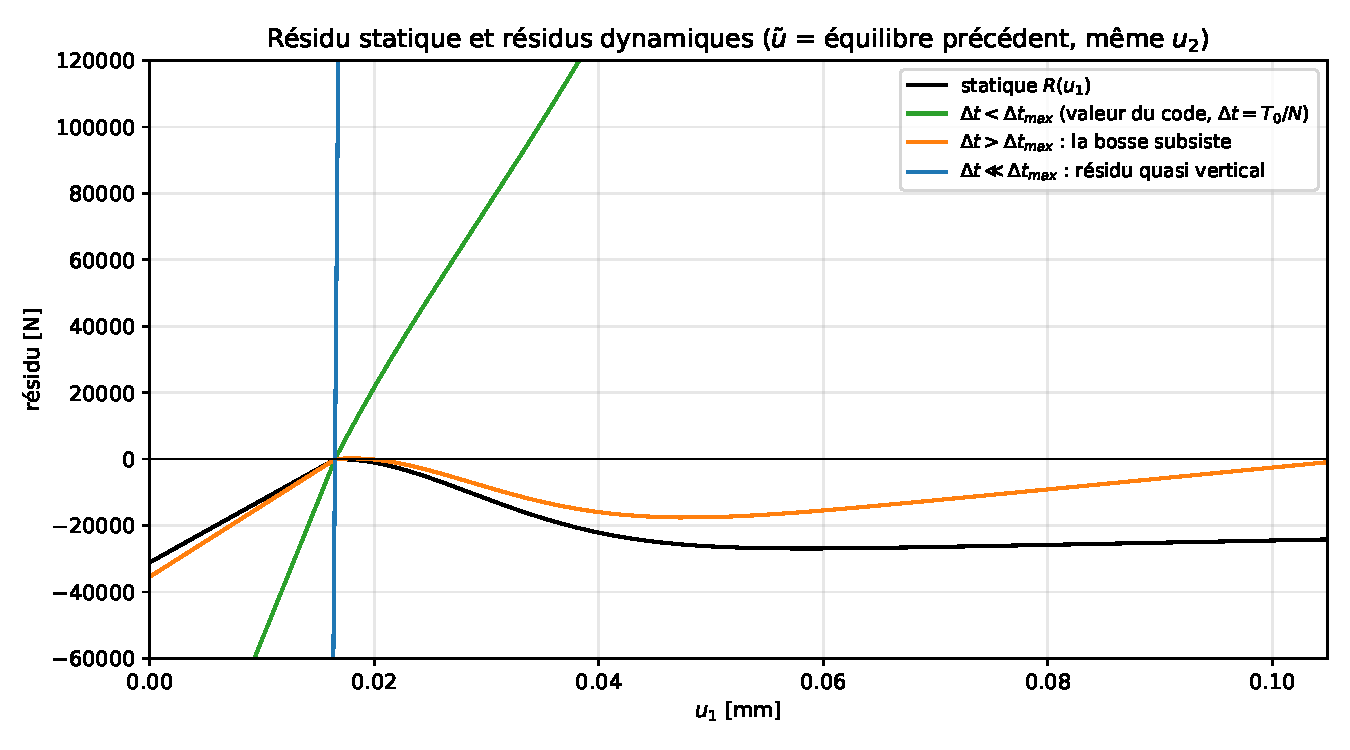
\includegraphics[width=.85\textwidth]{figures/explication_residu_dyn.pdf}
  \caption{Le terme d'inertie ajoute au résidu statique une droite de pente $m_1c_1$ passant par
  $\tilde u$. Dès que cette pente dépasse $1{,}27\cdot10^6$~N/mm, la bosse disparaît et Newton n'a
  plus qu'une racine.}
  \label{fig:resdyn}
\end{figure}

\begin{idee}
Pendant un pas de temps, la masse ne peut s'écarter de sa position prédite $\tilde u$ qu'en
payant une force d'inertie $m_1c_1(u_1-\tilde u)$. Tout se passe comme si un ressort numérique de
raideur $m_1/(\beta\Delta t^2)$ la retenait à $\tilde u$. Si ce ressort est plus raide que la
descente la plus raide du béton, le problème de chaque pas est bien posé. Le saut n'est pas
supprimé : il est \emph{étalé} sur plusieurs pas, pendant lesquels $\tilde u$ se déplace et
emporte le résidu avec lui.
\end{idee}

\subsection{Comment se déroule le saut en dynamique}
Au point limite, la racine du résidu dynamique s'écarte de l'équilibre statique ; la masse
acquiert une vitesse, $\tilde u$ au pas suivant est plus loin, et ainsi de suite : en quelques
dizaines de pas $u_1$ passe de $0{,}017$ à $0{,}47$~mm. L'énergie $|W| = 6{,}3$~J devient cinétique
(le code mesure $K_{\max} = 6{,}26$~J, la petite différence étant l'amortissement numérique).
Ensuite le ressort 1 est mort ($d = 1$, maintenu par $\kappa$), et la masse oscille librement sur
le ressort 2 autour de $u_2$ :
\begin{equation}
  m_1\ddot u_1 + k_2(u_1-u_2) = 0,\qquad T_{\text{libre}} = 2\pi\sqrt{\frac{m_1}{k_2}},\qquad
  \text{amplitude} = u_2^{\lim}-u_1^{\lim}.
\end{equation}
\begin{alamain}
$T_{\text{libre}} = 2\pi\sqrt{0{,}0274/65\,973} = 4{,}05$~ms (mesuré : 4,04~ms) ; amplitude $0{,}471-0{,}017 = 0{,}45$~mm.
\end{alamain}
La force $F_2 = k_2(u_2-u_1)$ oscille alors entre $\pm30$~kN : la barre d'acier passe en
compression à chaque demi-période (figure~\ref{fig:zoom}). Deux limites physiques du modèle
apparaissent ici : une barre $\varnothing20$ de 1~m flambe bien avant 30~kN de compression (charge
d'Euler 16~kN), et le béton rompu devrait reprendre de la raideur si la fissure se referme
($u_1 < 0$), ce qui n'arrive pas ici car l'amplitude ramène $u_1$ au plus à $0{,}017$~mm.

\begin{figure}[h]\centering
  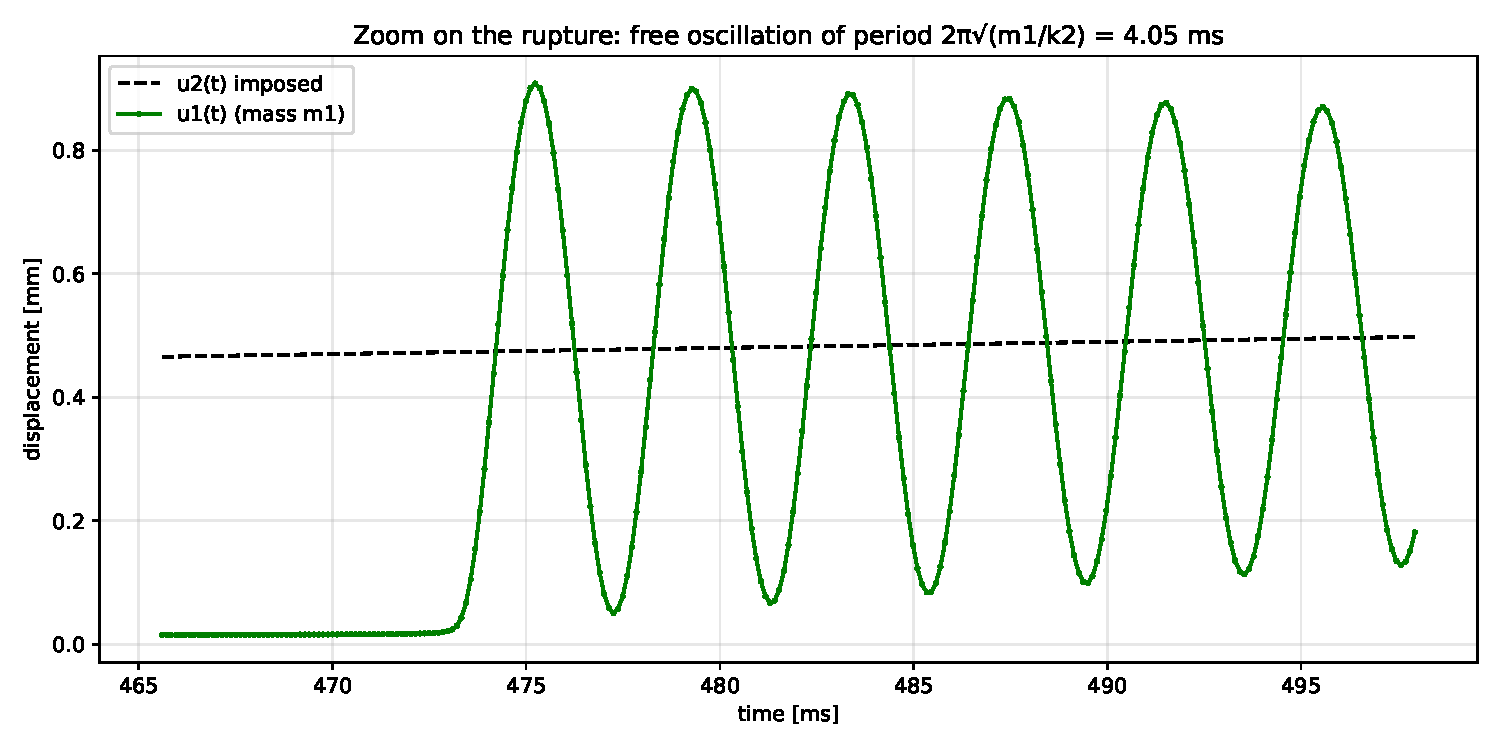
\includegraphics[width=.8\textwidth]{figures/rupture_zoom.pdf}
  \caption{Zoom sur la rupture dynamique : le noeud 1 rejoint $u_2$ en une demi-période puis
  oscille librement sur le ressort 2, avec une décroissance lente due à l'amortissement
  numérique du Newmark.}
  \label{fig:zoom}
\end{figure}

\subsection{Le choix de la vitesse de rampe}
Pour que la dynamique n'intervienne qu'au saut, la rampe doit être lente devant $T_0$ : ici
$0{,}6$~mm en $0{,}6$~s, soit mille périodes propres. Avant le point limite, la solution dynamique est
confondue avec la statique (la force d'inertie vaut $m_1\ddot u_1 \simeq 0$). Une vitesse réelle
d'essai (0,5~mm/min) demanderait $10^6$ pas ; 1~mm/s est un compromis.

\section{Synthèse}

\begin{center}
\begin{tabular}{@{}p{3.2cm}p{5.4cm}p{6.2cm}@{}}
\toprule
Méthode & Ce qu'elle donne & Comment elle traite le point limite\\
\midrule
Analytique & toute la branche $F(u_2)$, y compris le rebroussement & en paramétrant par $u_1$, on n'a jamais à inverser $R$\\
Statique NR & la réponse d'un essai piloté en déplacement idéal (saut vertical) & Newton cycle ; relance depuis $u_1 = u_2$\\
Dynamique Newmark + NR & la réponse physique (saut en quelques pas, oscillations) & l'inertie $m_1/(\beta\Delta t^2)$ rend le résidu monotone si $\Delta t < \Delta t_{\max}$\\
\bottomrule
\end{tabular}
\end{center}

\begin{alamain}
Vérifications à refaire soi-même, avec les valeurs attendues :
\begin{enumerate}[nosep]
  \item $k_1 = 3\cdot10^6$, $k_2 = 6{,}6\cdot10^4$~N/mm ; $k_2/k_1 = 0{,}022 < 0{,}446$ : snap-back.
  \item $\uc = 0{,}0233$~mm, $F_{\max} = 30$~kN à $u_1 = 0{,}0165$~mm et $u_2 = 0{,}471$~mm.
  \item Pente la plus raide de $F_1$ : $-0{,}446\,k_1 = -1{,}34\cdot10^6$~N/mm ; longueur critique de barre $49$~mm.
  \item Point limite : $x_{\lim} = 0{,}720$, $u_2^{\lim} = 0{,}4714$~mm ; rebroussement jusqu'à $u_2 = 0{,}063$~mm.
  \item Énergie au pic : 6,8~J dans l'acier, 0,25~J dans le béton ; énergie libérée $|W| = 6{,}3$~J.
  \item $T_0 = 0{,}594$~ms, $\Delta t_{\max} = 0{,}27$~ms, soit plus de 2,2 pas par période.
  \item $T_{\text{libre}} = 4{,}05$~ms, amplitude 0,45~mm, $F_2$ entre $\pm30$~kN.
\end{enumerate}
\end{alamain}

\end{document}
